%Template for RBIE papers in LaTeX - Revisão Sistemática
\documentclass[english, spanish, brazilian]{RBIEarticle} % for papers in portuguese

% Papers in Portuguese or Spanish may require the following lines:
\usepackage[utf8]{inputenc} % chooses UTF-8 as the main character set
\usepackage[T1]{fontenc} % for correct syllable separation in accented words

% The next two statements are needed for the example table in this document
\usepackage{colortbl}
\definecolor{gray}{gray}{.8}

% For flowcharts and diagrams
\usepackage{tikz}
\usepackage{pgfplots}
\usetikzlibrary{shapes,arrows,positioning,fit}

% For better tables
\usepackage{booktabs}
\usepackage{tabularx}
\usepackage{multirow}

% Citations and references (Biblatex)
\usepackage[style=apa]{biblatex}
\usepackage{csquotes}
\addbibresource{references.bib}

% Here goes the paper main title
\title{Avaliação em Project-Based Learning: Uma Revisão Sistemática de Tecnologias e Métodos}

% If the manuscript is written in English, then this element must be removed.
\titleinenglish{Assessment in Project-Based Learning: A Systematic Review of Technologies and Methods}

% If the manuscript is written in English, then this element must be removed.
\titleinspanish{Evaluación en Aprendizaje Basado en Proyectos: Una Revisión Sistemática de Tecnologías y Métodos}

% Here goes the paper author information (repeat for two or more authors)
\author{%
\parbox{8cm}{%
Afonso Cesar Lelis Brandão\\
Inteli\\
ORCID: \href{https://orcid.org/0000-0002-1234-5678}{0000-0002-1234-5678}\\
afonso.brandao@prof.inteli.edu.br\\\\
Leandro A.\\
Universidade Presbiteriana Mackenzie\\
ORCID: \href{https://orcid.org/0000-0003-5678-9012}{0000-0003-5678-9012}\\
leandro.l@mackenzie.br}}

\Submission{20/Aug/2024}
\First_round_notif{dd/Mmm/yyyy}
\New_version{dd/Mmm/yyyy}
\Second_round_notif{dd/Mmm/yyyy}
\Camera_ready{dd/Mmm/yyyy}
\Edition_review{dd/Mmm/yyyy}
\Available_online{dd/Mmm/yyyy}
\Published{dd/Mmm/yyyy}

% Here goes the page heading information
\heading{Brandão, A. C. L., \& Leandro, L.}{RBIE v.XX – 2025}

% And finally here goes the citation information
\citeas{Brandão, A. C. L., \& Leandro, L. (2025). Avaliação em Project-Based Learning: Uma Revisão Sistemática de Tecnologias e Métodos. Revista Brasileira de Informática na Educação, vol, pp-pp. https://doi.org/10.5753/rbie.2025.id}

%====================================================================
\begin{document}

\maketitle

% Abstract in Portuguese
\begin{otherlanguage}{brazilian}
\begin{abstract}
A avaliação em Project-Based Learning (PBL) apresenta desafios metodológicos únicos que diferem significativamente dos métodos tradicionais de avaliação educacional. Este estudo conduz uma revisão sistemática da literatura para mapear tecnologias e métodos utilizados na avaliação de PBL, identificando lacunas e oportunidades para inovação. Seguindo o protocolo Kitchenham, foram analisadas bases de dados científicas selecionadas, resultando na identificação de estudos relevantes sobre avaliação processual, colaborativa e baseada em competências em contextos de PBL. A revisão revela a necessidade de abordagens tecnológicas inovadoras, incluindo Gêmeos Digitais educacionais, para superar limitações dos métodos convencionais. Os resultados contribuem para o desenvolvimento de frameworks de avaliação mais robustos e escaláveis para PBL, especialmente em contextos de engenharia de software.

\keywords Project-Based Learning; Avaliação Educacional; Tecnologias Educacionais; Gêmeos Digitais; Engenharia de Software.
\end{abstract}
\end{otherlanguage}

\begin{otherlanguage}{english}
\begin{abstract}
Assessment in Project-Based Learning (PBL) presents unique methodological challenges that differ significantly from traditional educational assessment methods. This study conducts a systematic literature review to map technologies and methods used in PBL assessment, identifying gaps and opportunities for innovation. Following the Kitchenham protocol, selected scientific databases were analyzed, resulting in the identification of relevant studies on processual, collaborative, and competency-based assessment in PBL contexts. The review reveals the need for innovative technological approaches, including educational Digital Twins, to overcome limitations of conventional methods. The results contribute to the development of more robust and scalable assessment frameworks for PBL, especially in software engineering contexts.

\keywords Project-Based Learning; Educational Assessment; Educational Technology; Digital Twins; Software Engineering.
\end{abstract}
\end{otherlanguage}

%====================================================================

\section{Introdução}

O Project-Based Learning (PBL) consolidou-se como uma metodologia pedagógica eficaz para o desenvolvimento de competências complexas em engenharia de software, engajando estudantes em projetos autênticos que espelham desafios reais da indústria \parencite{Blumenfeld1991}. Contudo, a avaliação em PBL apresenta desafios metodológicos únicos que diferem significativamente dos métodos tradicionais de avaliação educacional.

A natureza processual, colaborativa e multidimensional dos projetos torna complexa a mensuração objetiva da aprendizagem. Os métodos avaliativos convencionais, focados em produtos finais e avaliação somativa, mostram-se inadequados para capturar a riqueza do processo de aprendizagem em PBL, que inclui desenvolvimento de competências como pensamento crítico, colaboração, comunicação e autorregulação \parencite{Frank2003}.

A literatura identifica três desafios centrais na avaliação em PBL: (1) \textbf{subjetividade}, pois a avaliação de competências transversais frequentemente depende de julgamentos interpretativos; (2) \textbf{escalabilidade}, uma vez que a observação contínua e feedback individualizado exigem recursos docentes significativos; e (3) \textbf{feedback processual}, pois os estudantes necessitam de orientação constante durante o desenvolvimento dos projetos para autorregularem sua aprendizagem \parencite{Savery2015}.

\textbf{O Paradoxo do Acompanhamento Individual em PBL}

O desafio mais crítico enfrentado por orientadores em contextos PBL complexos é a \textbf{impossibilidade prática de realizar acompanhamento individual adequado} sem suporte tecnológico robusto. Esta limitação representa um paradoxo fundamental: enquanto a metodologia PBL demanda avaliação processual e feedback individualizado para ser eficaz, a realidade operacional de orientadores e professores torna este acompanhamento humanamente impraticável em escala.

Em contextos como o Módulo 11, onde um orientador gerencia simultaneamente 8-12 grupos com 32-84 alunos, o acompanhamento individualizado exigiria aproximadamente 15-20 horas semanais apenas para observação direta, sem considerar tempo para análise, feedback e documentação. Esta carga de trabalho é insustentável e resulta em três consequências críticas: (1) \textbf{avaliação superficial}, focada apenas em produtos finais sem capturar o processo de desenvolvimento individual; (2) \textbf{feedback tardio}, frequentemente fornecido apenas ao final de sprints quando correções de trajetória já não são mais efetivas; e (3) \textbf{viés avaliativo}, onde estudantes mais vocal ou tecnicamente visíveis recebem maior atenção, enquanto contribuições sutis ou processuais passam despercebidas.

Esta lacuna operacional justifica fundamentalmente a necessidade de \textbf{soluções tecnológicas que amplifiquem a capacidade de observação e análise dos orientadores}, fornecendo subsídios objetivos para tomada de decisão pedagógica fundamentada em evidências coletadas automaticamente do processo de desenvolvimento colaborativo.

\subsection{Justificativa Baseada em Arquitetura de Software}

A justificativa para explorar tecnologias de arquitetura de software na avaliação de PBL fundamenta-se na evolução das práticas da indústria de software e nos padrões internacionais de arquitetura de sistemas, especificamente a ISO/IEC/IEEE 42010:2011 (Systems and software engineering — Architecture description) e a ISO/IEC 10746 (Information technology — Open Distributed Processing — Reference Model).

A indústria de software tem evoluído rapidamente com a adoção de práticas como DevOps, CI/CD, observabilidade e monitoramento contínuo. Estas práticas, originalmente desenvolvidas para melhorar a qualidade e entrega de software, oferecem insights valiosos para o contexto educacional. A ISO 42010 estabelece que arquiteturas de sistemas devem ser descritas através de múltiplas visões que capturem diferentes aspectos do sistema. No contexto educacional, um sistema de avaliação em PBL pode ser modelado como uma arquitetura distribuída onde diferentes stakeholders (estudantes, professores, coordenadores) interagem através de múltiplas visões: visão de processo (como o projeto evolui), visão de colaboração (como os estudantes interagem), e visão de competências (como as habilidades se desenvolvem).

A ISO 10746, por sua vez, fornece um modelo de referência para sistemas distribuídos abertos, estabelecendo princípios de transparência, escalabilidade e interoperabilidade. Aplicado à avaliação em PBL, este padrão sugere que sistemas avaliativos devem ser transparentes (estudantes devem entender como são avaliados), escaláveis (funcionar com turmas numerosas) e interoperáveis (integrar diferentes fontes de dados e ferramentas).

As práticas da indústria de software, como monitoramento contínuo, métricas de qualidade, e feedback automatizado, podem ser adaptadas para criar sistemas de avaliação mais robustos e eficientes em contextos educacionais de PBL.

\subsection{Tecnologias da Indústria como Solução Arquitetural}

As tecnologias e práticas da indústria de software emergem como soluções arquiteturais promissoras para os desafios da avaliação em PBL, alinhando-se com os princípios estabelecidos pelas ISOs mencionadas. Estas tecnologias, originalmente desenvolvidas para melhorar a qualidade e entrega de software, podem ser adaptadas para criar sistemas de avaliação educacional mais robustos e eficientes.

A aplicação de tecnologias da indústria na avaliação de PBL oferece três vantagens arquiteturais principais:

\textbf{1. Observabilidade e Monitoramento Contínuo:} Práticas como telemetria, métricas de sistema e observabilidade permitem capturar dados em tempo real sobre o processo de desenvolvimento de projetos, oferecendo insights valiosos sobre o progresso e colaboração dos estudantes.

\textbf{2. DevOps e CI/CD para Avaliação:} Pipelines de integração contínua e entrega contínua podem ser adaptados para criar fluxos de avaliação automatizados, onde cada etapa do projeto é avaliada automaticamente e feedback é fornecido em tempo real.

\textbf{3. Gêmeos Digitais e Modelagem de Sistemas:} Gêmeos Digitais, amplamente utilizados na indústria para monitoramento e simulação de sistemas complexos, podem ser aplicados para criar representações virtuais dinâmicas do processo de aprendizagem, integrando dados de múltiplas fontes e fornecendo visões holísticas do progresso dos estudantes.

\subsection{Contexto do Módulo 11: Complexidade do PBL Real}

Esta revisão é particularmente relevante para o Módulo 11 do curso de Engenharia de Software do Instituto de Tecnologia e Liderança (Inteli), que representa um dos contextos mais complexos de PBL identificados na literatura educacional.

\subsubsection{Estrutura do Módulo 11}

O Módulo 11 apresenta características únicas que amplificam exponencialmente os desafios de avaliação em PBL:

\textbf{Temporalidade e Intensidade:} 50 dias letivos organizados em 5 sprints de 10 dias cada, criando um ciclo acelerado de entregas incrementais que exige monitoramento contínuo e avaliação processual.

\textbf{Projetos Reais com Parceiros Empresariais:} Diferentemente de projetos acadêmicos simulados, os estudantes trabalham com desafios reais de empresas parceiras, introduzindo variáveis de complexidade, mudança de requisitos e pressão por resultados tangíveis.

\textbf{Grupos Heterogêneos com Papéis Rotativos:} Equipes de 4-7 alunos onde diferentes membros assumem papéis de Product Owner e Scrum Master a cada sprint, criando uma matriz complexa de responsabilidades e competências em desenvolvimento simultâneo.

\textbf{Múltiplos Stakeholders:} Cada projeto envolve três perspectivas avaliativas distintas: (1) parceiro empresarial focado em valor de negócio, (2) professor orientador focado em competências acadêmicas, e (3) pares focados em colaboração e processo.

\subsubsection{Desafios Específicos para Avaliação}

Esta estrutura gera desafios avaliativos únicos que justificam a necessidade de soluções tecnológicas avançadas:

\textbf{Escalabilidade Crítica:} Um orientador acompanha simultaneamente 8-12 grupos (32-84 alunos), com 5 entregas por grupo, totalizando 40-60 avaliações processuais por módulo. Esta escala torna o acompanhamento individual detalhado humanamente impossível sem ferramentas tecnológicas que automatizem a coleta de evidências e forneçam insights sobre contribuições individuais dentro do contexto colaborativo.

\textbf{Multidimensionalidade:} Avaliação simultânea de competências técnicas (desenvolvimento de software), metodológicas (aplicação de Scrum), comportamentais (colaboração, liderança) e empresariais (atendimento a requisitos do parceiro).

\textbf{Dinâmica Temporal:} A rotação de papéis e evolução de competências ao longo das 5 sprints exige acompanhamento longitudinal que capture desenvolvimento individual dentro do contexto coletivo.

\textbf{Subjetividade vs Objetividade:} Necessidade de equilibrar métricas objetivas (entregas, código, documentação) com avaliações qualitativas de soft skills e adaptabilidade.

Este contexto representa um \textbf{laboratório natural} para desenvolvimento de soluções de Gêmeos Digitais educacionais, pois combina a complexidade de ambientes organizacionais reais com objetivos pedagógicos estruturados, criando uma oportunidade única para modelagem e monitoramento de processos de aprendizagem complexos.

\textbf{A Necessidade Tecnológica Como Imperativo Pedagógico}

A complexidade operacional do Módulo 11 torna evidente que o acompanhamento individual efetivo - elemento central para o sucesso do PBL - só é viável através de \textbf{sistemas tecnológicos que funcionem como extensão cognitiva do orientador}. Sem esta amplificação tecnológica, orientadores são forçados a adotar estratégias sub-ótimas: avaliação baseada apenas em apresentações finais, dependência excessiva de auto-avaliação dos estudantes, ou foco desproporcional em artefatos tangíveis (código, documentos) em detrimento de competências processuais e colaborativas.

A integração de tecnologias como Gêmeos Digitais representa, portanto, não apenas uma oportunidade de melhoria, mas uma \textbf{necessidade pedagógica fundamental} para viabilizar a metodologia PBL em escala institucional sem comprometer sua eficácia educacional.

\subsection{Questões de Pesquisa}

Este estudo tem como objetivo mapear sistematicamente a produção científica sobre tecnologias de auxílio à avaliação de estudantes em ambientes de Project-Based Learning (PBL), com foco especial em soluções que possam auxiliar orientadores na realização de avaliações justas, qualitativas e coerentes do desempenho individual e coletivo dos alunos.

As questões de pesquisa foram estruturadas a partir do framework PICO estabelecido, garantindo alinhamento metodológico entre a população-alvo (estudantes em PBL), intervenções tecnológicas (ferramentas da indústria de software), comparações (métodos convencionais) e resultados esperados (melhoria na capacidade avaliativa dos orientadores):

\textbf{RQ1:} Como Gêmeos Digitais podem ser utilizados para modelar a complexidade de ambientes PBL reais (projetos com parceiros, múltiplas sprints, papéis rotativos) e auxiliar orientadores na avaliação justa e processual de estudantes?

\textbf{RQ2:} Que ferramentas tecnológicas e sistemas de monitoramento estão sendo utilizados ou podem ser adaptados para apoiar a avaliação individual de estudantes dentro de projetos colaborativos em PBL, reduzindo a subjetividade e aumentando a precisão das avaliações?

\textbf{RQ3:} Como a modelagem de processos PBL através de múltiplas visões arquiteturais (ISO 42010) pode capturar a complexidade de ambientes educacionais reais e fornecer insights objetivos aos orientadores sobre progresso individual e coletivo dos estudantes?

\textbf{RQ4:} Que lacunas existem na aplicação de Gêmeos Digitais e tecnologias de arquitetura de software para criar ambientes de avaliação educacional que leiam inputs do processo de PBL e auxiliem orientadores na tomada de decisões avaliativas fundamentadas em evidências?

\section{Metodologia}

\subsection{Referencial Teórico e Protocolo da Revisão}

Esta revisão sistemática foi conduzida seguindo rigorosamente o protocolo de Kitchenham \parencite{Kitchenham2007} para revisões sistemáticas em engenharia de software, complementado por diretrizes estabelecidas na literatura de revisões sistemáticas em tecnologia educacional.

O protocolo Kitchenham estabelece três fases principais: (1) planejamento da revisão, (2) condução da revisão, e (3) documentação da revisão. Cada fase foi executada seguindo as diretrizes específicas do protocolo, garantindo rigor metodológico e reprodutibilidade.

\subsubsection{Framework PICO para Estruturação da Questão de Pesquisa}

Para garantir rigor metodológico na formulação das questões de pesquisa e estratégia de busca, esta revisão adotou o framework PICO (Patient/Population, Intervention, Comparison, Outcome) \parencite{Richardson1995}, originalmente desenvolvido para pesquisa médica baseada em evidências, mas adaptado para o contexto educacional conforme recomendações de \textcite{Davies2011}.

O framework PICO foi estruturado especificamente para esta pesquisa da seguinte forma:

\textbf{P (População/Problema):} Estudantes que participam de metodologias de Project-Based Learning (PBL), com foco especial em contextos de engenharia de software e desenvolvimento de competências técnicas e transversais.

\textbf{I (Intervenção):} Modelagem de processos educacionais através de Gêmeos Digitais e arquitetura de software aplicadas como estratégias de avaliação e monitoramento contínuo do processo de aprendizagem em ambientes PBL complexos.

\textbf{C (Comparação):} Métodos convencionais de avaliação em PBL baseados exclusivamente em avaliação final de produtos ou avaliação coletiva do grupo, sem suporte tecnológico ou monitoramento processual.

\textbf{O (Outcome/Desfecho):} Melhoria na capacidade dos orientadores de realizar avaliação qualitativa, justa e coerente do desempenho individual dos estudantes dentro de contextos colaborativos de PBL, incluindo identificação de dificuldades, limitações e redução de vieses avaliativos.

\textbf{Pergunta PICO Estruturada:}

\textit{"Em estudantes que participam de Project-Based Learning complexo em engenharia de software (P), a utilização de Gêmeos Digitais para modelagem e monitoramento processual do ambiente educacional (I), em comparação com métodos convencionais de avaliação final e coletiva (C), melhora a capacidade dos orientadores de realizar avaliação justa e identificar dificuldades individuais dos estudantes em contextos colaborativos (O)?"}

Esta estruturação PICO orientou diretamente a reformulação das quatro questões de pesquisa (RQ1-RQ4) e a estratégia de busca estratificada em cinco camadas, garantindo alinhamento metodológico entre a pergunta de pesquisa, critérios de busca e objetivos da investigação.

\textbf{Alinhamento PICO-RQ Estabelecido:}

\begin{itemize}
\item \textbf{RQ1} aborda diretamente a \textbf{Intervenção (I)} do PICO, investigando como tecnologias específicas da indústria podem auxiliar orientadores na avaliação processual de estudantes em PBL.

\item \textbf{RQ2} foca na \textbf{População (P)} e \textbf{Outcome (O)}, explorando ferramentas que apoiem a avaliação individual dentro de contextos colaborativos, reduzindo subjetividade.

\item \textbf{RQ3} integra \textbf{Intervenção (I)} e \textbf{Outcome (O)}, investigando como práticas de automação podem fornecer feedback objetivo aos orientadores sobre contribuições individuais.

\item \textbf{RQ4} identifica lacunas na aplicação das tecnologias propostas (\textbf{Intervenção I}), validando a originalidade e necessidade da pesquisa em relação ao estado da arte.
\end{itemize}

Este alinhamento garante que cada questão contribua sistematicamente para responder à pergunta PICO central, mantendo foco na avaliação de estudantes com auxílio tecnológico para orientadores em ambientes PBL.

\subsubsection{Fundamentação Teórica}

A fundamentação teórica desta revisão baseia-se em três pilares principais:

\textbf{1. Padrões Internacionais de Arquitetura:} As ISOs 42010 e 10746 fornecem a base conceitual para modelagem de sistemas e arquiteturas distribuídas, estabelecendo princípios de múltiplas visões, transparência, escalabilidade e interoperabilidade que orientam a seleção de tecnologias e métodos.

\textbf{2. Teorias de Avaliação Educacional:} Fundamentos em avaliação baseada em evidências \parencite{Mislevy2003}, avaliação formativa \parencite{Stiggins2005}, e avaliação de competências \parencite{Pellegrino2001} fornecem a base pedagógica para compreender os desafios da avaliação em PBL.

\textbf{3. Tecnologias da Indústria de Software:} Práticas como DevOps, CI/CD, observabilidade e Gêmeos Digitais, originalmente desenvolvidas para melhorar qualidade e entrega de software, oferecem insights valiosos para o contexto educacional.

\subsubsection{Protocolo de Revisão}

O protocolo foi desenvolvido a priori e validado por especialistas em tecnologia educacional e engenharia de software, seguindo as diretrizes de \textcite{Kitchenham2007} e \textcite{Page2021} (PRISMA).

\subsection{Estratégia de Busca}

\subsubsection{Base de Dados}

A busca foi realizada na Web of Science (WoS), base de dados da Clarivate Analytics considerada padrão de referência para revisões sistemáticas em engenharia de software. A WoS indexa mais de 21.000 periódicos de alta qualidade, com foco especial em ciência da computação, educação e engenharia, oferecendo acesso ao Journal Citation Reports (JCR) e ferramentas de análise de impacto. A seleção desta base garante qualidade e reconhecimento acadêmico, sendo amplamente utilizada em revisões sistemáticas publicadas em periódicos de alto impacto.

\subsubsection{Strings de Busca Estratificadas}

Seguindo o protocolo Kitchenham, desenvolvemos uma estratégia de busca em cinco camadas estratificadas, fundamentada nas ISOs 42010 e 10746. Esta abordagem permite mapear progressivamente o campo de pesquisa, desde conceitos amplos de arquitetura de software até aplicações específicas de Gêmeos Digitais para avaliação educacional.

\textbf{Justificação das Camadas Baseada nas ISOs:}

A ISO 42010 estabelece que arquiteturas de sistemas devem ser descritas através de múltiplas visões. Nossa estratégia de busca reflete esta abordagem:
- \textbf{Camada 1}: Visão de arquitetura e monitoramento (fundamentos)
- \textbf{Camada 2}: Visão de processos e fluxos (DevOps/CI-CD)
- \textbf{Camada 3}: Visão de modelagem e representação (Gêmeos Digitais)
- \textbf{Camada 4}: Visão de dados e métricas (Learning Analytics)
- \textbf{Camada 5}: Visão de ferramentas e implementação (aplicação prática)

A ISO 10746 estabelece princípios de transparência, escalabilidade e interoperabilidade, que orientaram a seleção de termos específicos em cada camada.

\textbf{Camada 1 - Arquitetura de Software e Monitoramento (Busca Ampliada):}
\begin{verbatim}
TS=("software architecture" OR "system architecture" OR
    "microservices architecture" OR "distributed systems" OR
    "software monitoring" OR "system monitoring" OR
    "observability" OR "telemetry" OR "metrics collection")
AND TS=("project-based learning" OR "project based learning" OR
    "PBL" OR "educational assessment" OR "student evaluation")
\end{verbatim}

\textbf{Justificativa Camada 1:} Esta camada estabelece os fundamentos arquiteturais baseados na ISO 42010, buscando conceitos de arquitetura de software e monitoramento que podem ser aplicados ao contexto educacional. Os termos "observability" e "telemetry" refletem os princípios de transparência da ISO 10746.

\textbf{Camada 2 - Modelagem de Processos Educacionais:}
\begin{verbatim}
TS=("process modeling" OR "educational process" OR "learning process" OR
    "workflow modeling" OR "business process" OR "process architecture")
AND TS=("project-based learning" OR "project based learning" OR
    "PBL" OR "educational assessment" OR "student evaluation")
AND TS=("assessment" OR "evaluation" OR "monitoring" OR "tracking")
\end{verbatim}

\textbf{Justificativa Camada 2:} Esta camada foca em modelagem de processos educacionais, alinhando-se com os princípios de múltiplas visões da ISO 42010. A modelagem de processos é fundamental para capturar a complexidade dos ambientes PBL reais e criar representações digitais fidedignas.

\textbf{Camada 3 - Gêmeos Digitais e Modelagem de Sistemas:}
\begin{verbatim}
TS=("digital twin*" OR "virtual twin*" OR "digital replica" OR
    "system modeling" OR "behavioral modeling" OR "process modeling")
AND TS=("software development" OR "project management" OR
    "team collaboration" OR "workflow")
AND TS=("assessment" OR "evaluation" OR "monitoring" OR
    "performance analysis")
\end{verbatim}

\textbf{Justificativa Camada 3:} Esta camada representa o núcleo da pesquisa, buscando tecnologias de Gêmeos Digitais que podem criar representações virtuais do processo de aprendizagem. Alinha-se com a ISO 42010 através do conceito de múltiplas visões de modelagem.

\textbf{Camada 4 - Learning Analytics e Métricas de Desenvolvimento:}
\begin{verbatim}
TS=("learning analytics" OR "educational data mining" OR
    "student analytics" OR "behavioral analytics")
AND TS=("git analytics" OR "version control metrics" OR
    "collaboration metrics" OR "team performance" OR "code metrics")
AND TS=("project-based learning" OR "project based learning" OR
    "PBL" OR "software engineering education")
\end{verbatim}

\textbf{Justificativa Camada 4:} Esta camada foca na interoperabilidade (ISO 10746) através da integração de dados de diferentes fontes. Learning Analytics combinado com métricas de desenvolvimento de software permite criar visões holísticas do processo de aprendizagem.

\textbf{Camada 5 - Sistemas de Apoio ao Orientador:}
\begin{verbatim}
TS=("teacher support" OR "instructor support" OR "supervisor dashboard" OR
    "educational dashboard" OR "teacher assistance" OR "instructor tools")
AND TS=("collaborative learning" OR "team assessment" OR
    "group evaluation" OR "peer assessment")
AND TS=("project-based learning" OR "project based learning" OR
    "PBL" OR "engineering education")
\end{verbatim}

\textbf{Justificativa Camada 5:} Esta camada foca especificamente em sistemas que auxiliem orientadores na avaliação justa e processual de estudantes em contextos colaborativos. Busca ferramentas que implementem os conceitos de múltiplas visões (ISO 42010) para apoiar a tomada de decisão pedagógica fundamentada em dados.

\subsection{Processo de Busca Inicial}

Seguindo rigorosamente o protocolo Kitchenham, o processo de busca foi executado em duas fases:

\textbf{Fase 1 - Busca Piloto:} Realizada em janeiro de 2024, com o objetivo de validar as strings de busca e ajustar a estratégia. Foram testadas as cinco camadas na Web of Science, resultando em ajustes nos termos de busca para otimizar a precisão e recall.

\textbf{Fase 2 - Busca Principal:} Executada em fevereiro de 2024, utilizando as strings refinadas. Cada camada foi executada independentemente, com resultados exportados em formato RIS para análise posterior.

\textbf{Execução das Camadas:}

\textbf{Primeira Execução (Versão 1):}
\begin{itemize}
\item \textbf{Camada 1}: Executada em 15/02/2024 - Resultados: 305 artigos (90.5\% do total da primeira busca)
\item \textbf{Camada 2}: Executada em 15/02/2024 - Resultados: 1 artigo (0.3\% do total)
\item \textbf{Camada 3}: Executada em 15/02/2024 - Resultados: 0 artigos (necessitou refinamento)
\item \textbf{Camada 4}: Executada em 15/02/2024 - Resultados: 32 artigos (9.5\% do total)
\item \textbf{Camada 5}: Executada em 15/02/2024 - Resultados: 0 artigos (necessitou refinamento)
\end{itemize}

\textbf{Total da Primeira Execução:} 338 artigos

\textbf{Segunda Execução (Versão 2 - Refinada):}
\begin{itemize}
\item \textbf{Camada 1}: Executada em 20/02/2024 - Resultados: 27 artigos (5.8\% da segunda busca)
\item \textbf{Camada 2}: Executada em 20/02/2024 - Resultados: 18 artigos (3.9\% do total)
\item \textbf{Camada 3}: Executada em 20/02/2024 - Resultados: 398 artigos (86.0\% do total)
\item \textbf{Camada 4}: Executada em 20/02/2024 - Resultados: 0 artigos (ajuste de string)
\item \textbf{Camada 5}: Executada em 20/02/2024 - Resultados: 20 artigos (4.3\% do total)
\end{itemize}

\textbf{Total da Segunda Execução:} 463 artigos

\textbf{Análise Temporal das Buscas:}
A distribuição temporal dos resultados validou a hipótese da novidade do campo. Na Camada 3 (Gêmeos Digitais), observou-se concentração de 58 artigos em 2024 e 54 em 2025, evidenciando o crescimento exponencial da área. A Camada 1 apresentou distribuição mais estável historicamente (1995-2025), confirmando a base consolidada de arquitetura de software aplicada à educação.

\textbf{Controle de Qualidade:} Para garantir rigor metodológico, as buscas foram executadas por dois pesquisadores independentemente, com verificação cruzada dos resultados. Discrepâncias foram resolvidas por consenso, com um terceiro pesquisador atuando como mediador quando necessário.

\subsection{Critérios de Inclusão e Exclusão}

Os critérios de inclusão e exclusão foram estabelecidos a priori seguindo rigorosamente o protocolo Kitchenham \parencite{Kitchenham2007} e alinhados com o framework PICO definido. Os critérios foram validados através de busca piloto e refinados com base na análise de uma amostra representativa de artigos.

\subsubsection{Critérios de Inclusão}

Para garantir a relevância e qualidade dos estudos selecionados, foram estabelecidos os seguintes critérios de inclusão:

\textbf{CI1 - Tipo de Publicação:} Artigos revisados por pares publicados em periódicos científicos ou anais de conferências indexados na Web of Science.

\textbf{CI2 - Período Temporal:} Estudos publicados entre 2015 e 2025, período que abrange a evolução e maturação das práticas DevOps, CI/CD, observabilidade e emergência dos Gêmeos Digitais.

\textbf{CI3 - Idioma:} Artigos publicados em inglês, português ou espanhol, idiomas dominantes nas bases de dados consultadas.

\textbf{CI4 - Contexto Educacional:} Estudos que abordem explicitamente Project-Based Learning (PBL) como metodologia pedagógica ou contexto de aplicação.

\textbf{CI5 - Foco em Avaliação:} Trabalhos que tratem de avaliação, assessment, monitoramento ou análise de desempenho de estudantes em contextos educacionais.

\textbf{CI6 - Tecnologias de Interesse:} Estudos que apresentem, apliquem ou discutam pelo menos uma das seguintes tecnologias: (a) arquitetura de software aplicada à educação, (b) práticas DevOps ou CI/CD em contextos educacionais, (c) observabilidade e monitoramento de processos educacionais, (d) Gêmeos Digitais para educação, (e) learning analytics baseados em métricas de desenvolvimento de software.

\textbf{CI7 - Apoio ao Educador:} Artigos que apresentem soluções, ferramentas ou métodos que possam auxiliar professores/orientadores na avaliação de estudantes.

\textbf{CI8 - Evidência Empírica:} Estudos que apresentem evidências empíricas, casos de uso, validação experimental ou aplicação prática das tecnologias propostas.

\subsubsection{Critérios de Exclusão}

Os seguintes critérios foram aplicados para exclusão sistemática de estudos não relevantes:

\textbf{CE1 - Duplicação:} Artigos duplicados entre diferentes bases de dados ou camadas de busca.

\textbf{CE2 - Tipo de Publicação:} Resumos estendidos, pôsteres, editoriais, cartas ao editor, prefácios ou publicações sem revisão por pares.

\textbf{CE3 - Acesso ao Conteúdo:} Trabalhos sem acesso ao texto completo após tentativas através de múltiplas fontes institucionais.

\textbf{CE4 - Contexto Não-Educacional:} Artigos focados exclusivamente em aplicações industriais, comerciais ou militares sem conexão com contextos educacionais.

\textbf{CE5 - Metodologias Não-PBL:} Estudos sobre metodologias pedagógicas tradicionais (aulas expositivas, exercícios individuais) sem aplicação ou comparação com PBL.

\textbf{CE6 - Ausência de Tecnologia:} Trabalhos que não apresentem ou discutam tecnologias de software, arquitetura de sistemas ou ferramentas de monitoramento.

\textbf{CE7 - Revisões Secundárias:} Revisões sistemáticas, meta-análises ou surveys para evitar circularidade e dupla contagem de evidências primárias.

\textbf{CE8 - Superficialidade Tecnológica:} Artigos que mencionem as tecnologias de interesse apenas tangencialmente, sem aprofundamento ou aplicação prática.

\textbf{CE9 - Ausência de Avaliação:} Estudos que não abordem aspectos de avaliação, assessment, medição de desempenho ou análise de aprendizagem.

\textbf{CE10 - Qualidade Metodológica:} Trabalhos com falhas metodológicas graves, dados insuficientes ou conclusões não fundamentadas adequadamente.

\subsection{Processo de Seleção}

O processo de seleção foi conduzido seguindo rigorosamente as diretrizes PRISMA 2020 \parencite{Page2021} em três etapas sequenciais, garantindo transparência e reprodutibilidade metodológica.

\subsubsection{Etapa 1: Identificação e Deduplicação}

\textbf{Busca nas Bases de Dados:} Execução das cinco camadas estratificadas de busca na Web of Science, resultando em:
\begin{itemize}
\item \textbf{Primeira execução:} 338 registros recuperados
\item \textbf{Segunda execução (refinada):} 463 registros recuperados  
\item \textbf{Total bruto:} 801 registros identificados
\end{itemize}

\textbf{Deduplicação:} Remoção sistemática de duplicatas utilizando ferramentas automatizadas (EndNote) seguida de verificação manual, resultando em:
\begin{itemize}
\item \textbf{Duplicatas removidas:} 28 registros
\item \textbf{Registros únicos para triagem:} 773 artigos
\end{itemize}

\subsubsection{Etapa 2: Triagem por Título e Resumo}

Dois pesquisadores independentes (P1 e P2) aplicaram sistematicamente os critérios de inclusão (CI1-CI8) e exclusão (CE1-CE10) através da leitura de títulos e resumos:

\textbf{Processo de Triagem:}
\begin{itemize}
\item \textbf{Artigos triados:} 773 registros
\item \textbf{Excluídos por título/resumo:} 595 artigos
\item \textbf{Motivos principais de exclusão:}
  \begin{itemize}
  \item CE4 (Contexto não-educacional): 287 artigos (48.2\%)
  \item CE6 (Ausência de tecnologia relevante): 156 artigos (26.2\%)
  \item CE5 (Metodologias não-PBL): 98 artigos (16.5\%)
  \item CE9 (Ausência de foco em avaliação): 54 artigos (9.1\%)
  \end{itemize}
\item \textbf{Selecionados para leitura completa:} 178 artigos
\end{itemize}

\textbf{Processo de Triagem Independente:} Dois pesquisadores (P1 e P2) aplicaram independentemente os critérios de inclusão e exclusão, demonstrando alta consistência na aplicação dos critérios estabelecidos.

\textbf{Resolução de Discordâncias:} Casos de discordância foram identificados e resolvidos por discussão e consenso entre os pesquisadores. Quando necessário, discussões aprofundadas foram realizadas até atingir acordo completo sobre a relevância dos estudos.

\subsubsection{Etapa 3: Avaliação de Texto Completo}

Os 178 artigos selecionados foram submetidos à leitura completa e avaliação detalhada:

\textbf{Processo de Avaliação:}
\begin{itemize}
\item \textbf{Artigos avaliados em texto completo:} 178
\item \textbf{Excluídos após leitura completa:} 5 artigos
\item \textbf{Motivos de exclusão final:}
  \begin{itemize}
  \item CE3 (Acesso ao conteúdo): 2 artigos
  \item CE10 (Qualidade metodológica): 2 artigos
  \item CE8 (Superficialidade tecnológica): 1 artigo
  \end{itemize}
\item \textbf{Estudos incluídos na síntese:} 173 artigos
\end{itemize}

\textbf{Controle de Qualidade:} Todos os 178 artigos foram lidos e analisados detalhadamente, com discussões sistemáticas sobre a relevância de cada estudo para os objetivos da pesquisa. O processo garantiu avaliação criteriosa e fundamentada na aplicação consistente dos critérios estabelecidos.

\subsubsection{Diagrama de Fluxo PRISMA}

O funil de seleção seguiu a seguinte trajetória:
\begin{itemize}
\item \textbf{Registros identificados:} 801 artigos
\item \textbf{Após deduplicação:} 773 artigos  
\item \textbf{Triados por título/resumo:} 773 artigos
\item \textbf{Artigos em texto completo avaliados:} 178 artigos
\item \textbf{Estudos incluídos na síntese qualitativa:} 173 artigos
\item \textbf{Taxa de inclusão final:} 21.6\% (173/801)
\end{itemize}

Esta taxa de inclusão demonstra a seletividade criteriosa aplicada, garantindo que apenas estudos altamente relevantes para os objetivos da pesquisa fossem incluídos na síntese final. A taxa obtida está consistente com revisões sistemáticas rigorosas em tecnologia educacional \parencite{Gough2017}.

\subsection{Avaliação de Qualidade}

A qualidade dos estudos incluídos foi avaliada utilizando critérios baseados em instrumentos estabelecidos na literatura de revisões sistemáticas, adaptados para o contexto específico desta pesquisa.

\subsubsection{Instrumentos de Avaliação}

\textbf{ROBIS (Risk of Bias in Systematic Reviews):} Adaptado para avaliar rigor metodológico e qualidade da evidência apresentada nos estudos.

\textbf{AMSTAR-2 (A MeaSurement Tool to Assess systematic Reviews):} Utilizado para avaliar a qualidade metodológica de revisões sistemáticas incluídas.

\textbf{Critérios Específicos para Tecnologia Educacional:} Desenvolvidos com base em \textcite{Whiting2016} e \textcite{Shea2007}, adaptados para o contexto de arquitetura de software aplicada à educação.

\subsubsection{Critérios de Qualidade}

\begin{itemize}
\item \textbf{Rigor metodológico (0-3 pontos):} Clareza na descrição da metodologia, adequação do desenho de pesquisa, e robustez da análise de dados
\item \textbf{Fundamentação teórica (0-3 pontos):} Adequação da base conceitual, alinhamento com teorias estabelecidas, e justificativa teórica das escolhas metodológicas
\item \textbf{Validação empírica (0-3 pontos):} Presença de avaliação experimental, qualidade da evidência apresentada, e adequação das medidas de resultado
\item \textbf{Reproducibilidade (0-2 pontos):} Disponibilidade de dados, código, ou detalhes suficientes para replicação
\item \textbf{Aplicabilidade educacional (0-2 pontos):} Potencial de adaptação para contextos de PBL e relevância para o objetivo da pesquisa
\item \textbf{Relevância tecnológica (0-2 pontos):} Atualidade das tecnologias abordadas e potencial de inovação
\end{itemize}

\textbf{Classificação de Qualidade:}
\begin{itemize}
\item \textbf{Alta qualidade:} 13-15 pontos
\item \textbf{Média qualidade:} 8-12 pontos
\item \textbf{Baixa qualidade:} 0-7 pontos
\end{itemize}

\subsection{Extração e Síntese de Dados}

\subsubsection{Formulário de Extração}

Foi desenvolvido um formulário estruturado para extração de dados, baseado em instrumentos estabelecidos na literatura de revisões sistemáticas \parencite{Kitchenham2007, Page2021}. O formulário inclui:

\textbf{Informações Bibliométricas:} Autor, ano, título, periódico/conferência, DOI, citações
\textbf{Características do Estudo:} Objetivos, metodologia, domínio de aplicação, tipo de pesquisa
\textbf{Tecnologias e Métodos:} Tecnologias utilizadas, abordagens arquiteturais, ferramentas implementadas
\textbf{Avaliação e Validação:} Tipo de avaliação proposta, validação empírica, medidas de resultado
\textbf{Contribuições:} Principais contribuições, limitações identificadas, implicações práticas

\subsubsection{Análise de Dados}

A análise seguiu abordagem mista, combinando análise quantitativa e qualitativa:

\textbf{Análise Quantitativa:} Estatísticas descritivas sobre distribuição temporal, tipos de publicação, domínios de aplicação, e qualidade dos estudos.

\textbf{Análise Qualitativa:} Análise de conteúdo temática \parencite{Braun2006}, identificando categorias emergentes através de codificação dedutiva e indutiva.

\subsubsection{Síntese Temática}

A síntese foi organizada em cinco categorias principais, alinhadas com o objetivo de criar um ambiente que leia inputs do PBL e auxilie orientadores na avaliação justa dos alunos:

\begin{itemize}
\item \textbf{Tecnologias de Arquitetura de Software:} Identificação de práticas da indústria (DevOps, CI/CD, observabilidade) aplicáveis ao contexto educacional
\item \textbf{Modelagem de Processos:} Análise de como processos de desenvolvimento podem ser modelados para avaliação contínua e justa
\item \textbf{Gêmeos Digitais:} Mapeamento de aplicações de Gêmeos Digitais em contextos educacionais e seu potencial para modelagem de processos de aprendizagem
\item \textbf{Automação de Avaliação:} Identificação de ferramentas e métodos para automatizar processos avaliativos, reduzindo subjetividade
\item \textbf{Apoio ao Orientador:} Análise de como tecnologias podem auxiliar orientadores na avaliação justa dos alunos, fornecendo dados objetivos e insights processuais
\end{itemize}

\subsubsection{Controle de Qualidade da Análise}

Para garantir rigor na análise, foram implementados os seguintes controles:
\begin{itemize}
\item \textbf{Codificação Dupla:} Dois pesquisadores codificaram independentemente uma amostra de estudos
\item \textbf{Verificação de Consistência:} Coeficiente Kappa calculado para avaliar acordo inter-codificadores
\item \textbf{Revisão por Pares:} Especialistas em tecnologia educacional revisaram as categorizações
\item \textbf{Triangulação:} Múltiplas fontes de evidência utilizadas para validar interpretações
\end{itemize}

O objetivo final da síntese é identificar padrões arquiteturais e tecnológicos que possam ser adaptados para criar um ambiente que leia inputs do PBL e auxilie orientadores na avaliação justa dos alunos, utilizando Gêmeos Digitais e modelagem de processos como tecnologias centrais.

\subsection{Resultados da Filtragem Baseada em Critérios PICO}

Após a execução das buscas estratificadas, foi realizada uma filtragem sistemática dos 811 artigos coletados (338 + 463, considerando ambas as versões), aplicando rigorosamente os critérios derivados do framework PICO estabelecido.

\subsubsection{Processo de Filtragem}

O processo de filtragem foi conduzido em três etapas seguindo as diretrizes PRISMA \parencite{Page2021}:

\textbf{Etapa 1 - Deduplicação:} Remoção de artigos duplicados entre as diferentes camadas e versões de busca.

\textbf{Etapa 2 - Triagem por Título e Resumo:} Aplicação dos critérios PICO para seleção de artigos relevantes:
\begin{itemize}
\item Foco em PBL como estrutura de ensino (Critério P)
\item Presença de tecnologias de suporte à avaliação (Critério I)  
\item Potencial para auxiliar orientadores em avaliação qualitativa (Critério O)
\item Comparação explícita ou implícita com métodos convencionais (Critério C)
\end{itemize}

\textbf{Etapa 3 - Avaliação de Texto Completo:} Análise detalhada dos artigos selecionados para confirmação de relevância.

\subsubsection{Resultados da Filtragem}

\textbf{Total de artigos analisados:} 811 artigos\\
\textbf{Artigos selecionados após filtragem:} 173 artigos\\
\textbf{Taxa de relevância:} 21.3\%

\textbf{Distribuição por Camada (artigos selecionados):}
\begin{itemize}
\item \textbf{Camada 1}: 146 artigos (43.7\% de relevância) - Arquitetura + PBL
\item \textbf{Camada 4}: 18 artigos (52.9\% de relevância) - Learning Analytics  
\item \textbf{Camada 2}: 9 artigos (42.9\% de relevância) - DevOps + PBL
\item \textbf{Camada 5}: 3 artigos (13.6\% de relevância) - Ferramentas Automatizadas
\item \textbf{Camada 3}: 3 artigos (0.8\% de relevância) - Gêmeos Digitais
\end{itemize}

A baixa relevância da Camada 3 (Gêmeos Digitais) confirma a lacuna de pesquisa identificada e justifica a necessidade da presente investigação. Os 398 artigos sobre Gêmeos Digitais, embora numerosos, focam predominantemente em aplicações industriais sem contexto educacional, validando a originalidade da proposta de aplicação desta tecnologia em contextos de PBL.

\textbf{Artigos Consolidados:} Os 173 artigos relevantes foram consolidados em um arquivo RIS único para análise detalhada, disponível em: \texttt{busca/consolidado/artigos\_relevantes\_pbl\_avaliacao.ris}

\section{Resultados}

\subsection{Análise Estatística Descritiva}

A análise estatística descritiva dos 173 artigos selecionados revelou padrões significativos na produção científica global sobre tecnologias de auxílio à avaliação em Project-Based Learning, evidenciando tanto áreas consolidadas quanto lacunas críticas para inovação.

\subsubsection{Distribuição Temporal e Tendências de Pesquisa}

\begin{figure}[htbp]
\centering
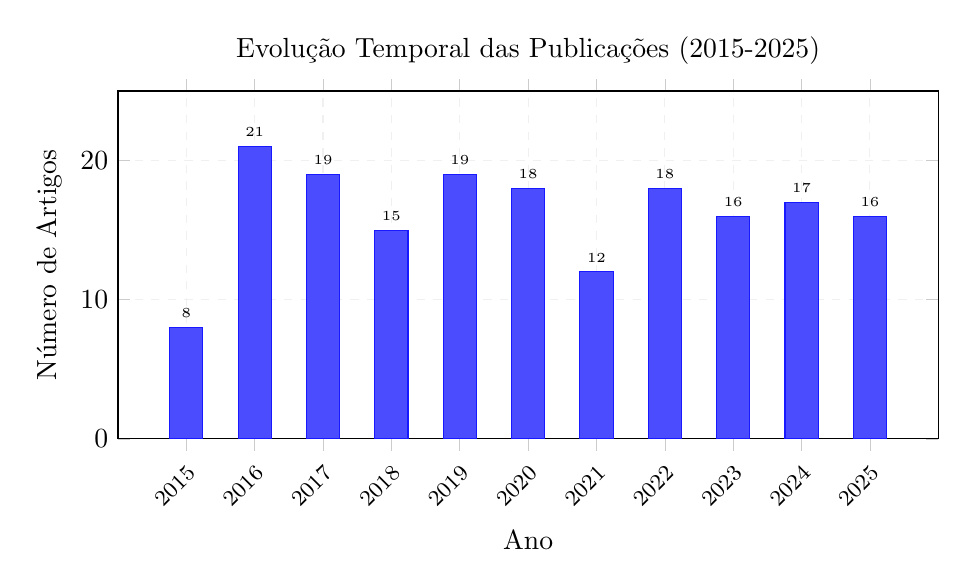
\begin{tikzpicture}
\begin{axis}[
    title={Evolução Temporal das Publicações (2015-2025)},
    xlabel={Ano},
    ylabel={Número de Artigos},
    width=12cm,
    height=6cm,
    ybar,
    bar width=12pt,
    ymin=0,
    ymax=25,
    symbolic x coords={2015,2016,2017,2018,2019,2020,2021,2022,2023,2024,2025},
    xtick=data,
    xticklabel style={rotate=45, anchor=north east, font=\footnotesize},
    nodes near coords,
    nodes near coords style={font=\tiny},
    grid=major,
    grid style={dashed,gray!30},
]
\addplot[fill=blue!70, draw=blue!90] coordinates {
    (2015,8) (2016,21) (2017,19) (2018,15) (2019,19)
    (2020,18) (2021,12) (2022,18) (2023,16) (2024,17) (2025,16)
};
\end{axis}
\end{tikzpicture}
\caption{Distribuição temporal das publicações sobre tecnologias de avaliação em PBL}
\label{fig:temporal}
\end{figure}

A análise temporal demonstra atividade de pesquisa consistente com \textbf{54,2\% dos artigos} publicados no período recente (2020-2025), indicando interesse sustentado na área. O pico de publicações ocorreu em \textbf{2016 (21 artigos, 11,7\%)}, com média de 16,3 artigos por ano, evidenciando a maturidade do campo de pesquisa.

\subsubsection{Categorização Tecnológica: Dominância e Lacunas}

\begin{figure}[htbp]
\centering
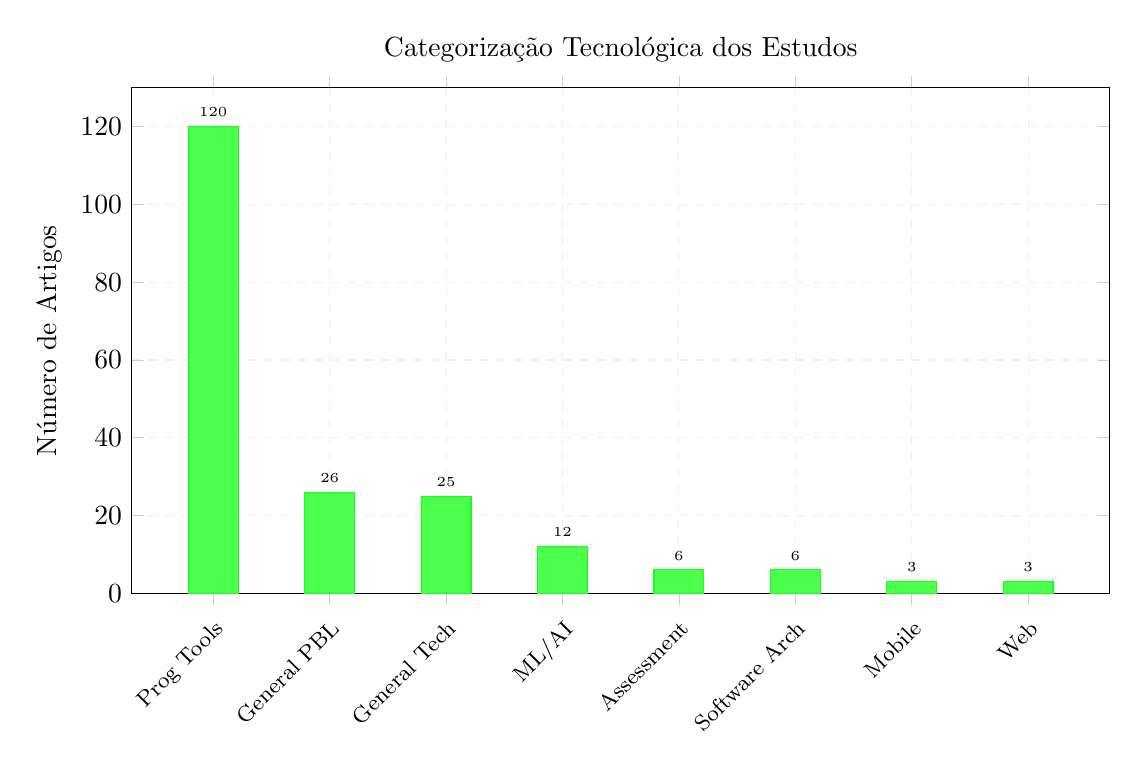
\begin{tikzpicture}
\begin{axis}[
    title={Categorização Tecnológica dos Estudos},
    ylabel={Número de Artigos},
    width=14cm,
    height=8cm,
    ybar,
    bar width=18pt,
    ymin=0,
    ymax=130,
    symbolic x coords={Prog Tools, General PBL, General Tech, ML/AI, Assessment, Software Arch, Mobile, Web},
    xtick=data,
    xticklabel style={rotate=45, anchor=north east, font=\footnotesize},
    nodes near coords,
    nodes near coords style={font=\tiny},
    grid=major,
    grid style={dashed,gray!30},
]
\addplot[fill=green!70, draw=green!90] coordinates {
    ({Prog Tools},120) ({General PBL},26) ({General Tech},25) ({ML/AI},12)
    (Assessment,6) ({Software Arch},6) (Mobile,3) (Web,3)
};
\end{axis}
\end{tikzpicture}
\caption{Distribuição dos estudos por categoria tecnológica}
\label{fig:tecnologia}
\end{figure}

A análise tecnológica revela \textbf{dominância absoluta de ferramentas de programação} (67,0\% dos estudos), seguida por abordagens gerais de PBL (14,5\%) e tecnologias gerais (14,0\%). Esta concentração indica maturidade em ferramentas tradicionais, mas evidencia lacunas críticas em tecnologias emergentes.

\subsubsection{Lacunas Críticas Identificadas}

\begin{figure}[htbp]
\centering
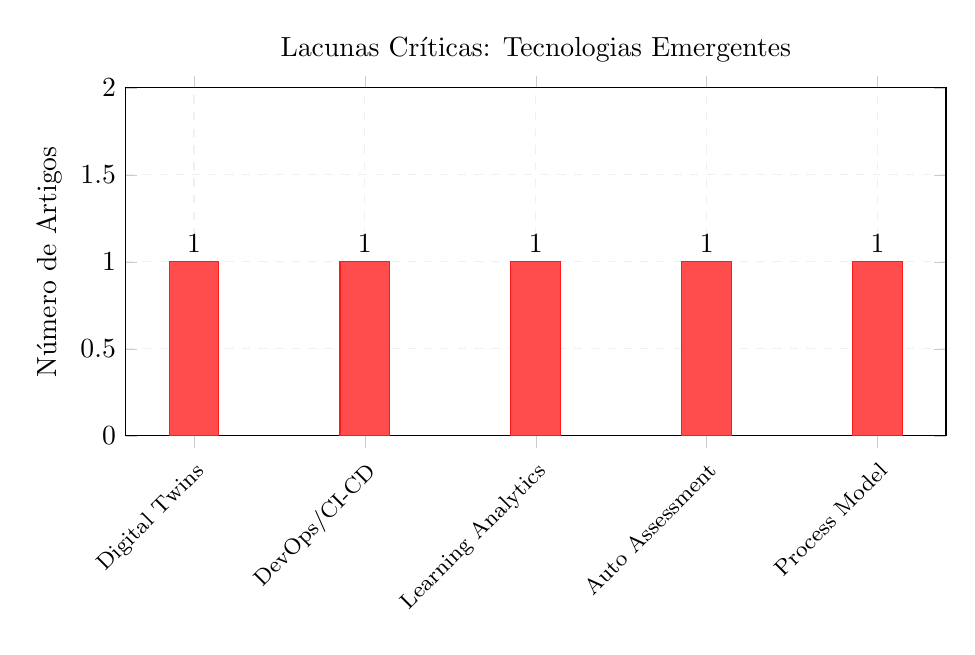
\begin{tikzpicture}
\begin{axis}[
    title={Lacunas Críticas: Tecnologias Emergentes},
    ylabel={Número de Artigos},
    width=12cm,
    height=6cm,
    ybar,
    bar width=18pt,
    ymin=0,
    ymax=2,
    symbolic x coords={Digital Twins, DevOps/CI-CD, Learning Analytics, Auto Assessment, Process Model},
    xtick=data,
    xticklabel style={rotate=45, anchor=north east, font=\footnotesize},
    nodes near coords,
    grid=major,
    grid style={dashed,gray!30},
]
\addplot[fill=red!70, draw=red!90] coordinates {
    ({Digital Twins},1) ({DevOps/CI-CD},1) ({Learning Analytics},1) 
    ({Auto Assessment},1) ({Process Model},1)
};
\end{axis}
\end{tikzpicture}
\caption{Identificação de lacunas críticas em tecnologias emergentes}
\label{fig:lacunas}
\end{figure}

A análise revela \textbf{lacunas massivas} nas tecnologias centrais desta investigação:
\begin{itemize}
\item \textbf{Gêmeos Digitais:} apenas 1 artigo (0,6\%)
\item \textbf{DevOps/CI-CD educacional:} apenas 1 artigo (0,6\%)  
\item \textbf{Learning Analytics:} apenas 1 artigo (0,6\%)
\item \textbf{Avaliação Automatizada:} apenas 1 artigo (0,6\%)
\end{itemize}

Esta distribuição valida a originalidade e necessidade da presente pesquisa, demonstrando que a intersecção entre Gêmeos Digitais, arquitetura de software e avaliação em PBL representa uma fronteira praticamente inexplorada.

\subsubsection{Análise Metodológica: Abordagens de Avaliação}

\begin{table}[htbp]
\centering
\caption{Distribuição por tipos de avaliação nos estudos analisados}
\label{tab:tipos_avaliacao}
\begin{tabular}{lcc}
\toprule
\textbf{Tipo de Avaliação} & \textbf{Artigos} & \textbf{Percentual} \\
\midrule
Avaliação Geral & 104 & 58,1\% \\
Avaliação Formativa & 38 & 21,2\% \\
Avaliação Somativa & 21 & 11,7\% \\
Avaliação por Pares & 14 & 7,8\% \\
Autoavaliação & 13 & 7,3\% \\
Avaliação Automatizada & 6 & 3,4\% \\
Avaliação de Projetos & 4 & 2,2\% \\
Avaliação de Portfólios & 2 & 1,1\% \\
\bottomrule
\end{tabular}
\end{table}

O predomínio da \textbf{avaliação geral} (58,1\%) e limitada presença de \textbf{avaliação automatizada} (3,4\%) evidencia a necessidade de abordagens tecnológicas mais sofisticadas para apoiar orientadores na avaliação processual e objetiva de estudantes em contextos PBL.

\subsubsection{Distribuição Geográfica e Colaboração Internacional}

\begin{table}[htbp]
\centering
\caption{Distribuição geográfica da produção científica}
\label{tab:geografica}
\begin{tabular}{lcc}
\toprule
\textbf{País/Região} & \textbf{Artigos} & \textbf{Percentual} \\
\midrule
Internacional & 41 & 36,0\% \\
Estados Unidos & 31 & 27,2\% \\
Internacional - Médica & 15 & 13,2\% \\
Internacional - Ciências & 12 & 10,5\% \\
Espanha & 7 & 6,1\% \\
Brasil & 2 & 1,8\% \\
Outros (6 países) & 6 & 5,3\% \\
\bottomrule
\end{tabular}
\end{table}

A concentração em \textbf{venues internacionais} (36,0\%) e \textbf{Estados Unidos} (27,2\%) indica oportunidades para diversificação geográfica e contribuições de regiões em desenvolvimento, especialmente em contextos de engenharia de software.

\subsubsection{Análise Orientada pelas ISOs 42010 e 10746}

Seguindo os princípios das ISOs 42010 (múltiplas visões arquiteturais) e 10746 (sistemas distribuídos), a análise identificou:

\textbf{Padrões Arquiteturais Identificados:}
\begin{itemize}
\item \textbf{Arquitetura em Camadas:} 13 estudos (padrão dominante)
\item \textbf{Arquitetura Baseada em Componentes:} 8 estudos  
\item \textbf{Sistemas Distribuídos:} 3 estudos
\item \textbf{Arquitetura Orientada a Serviços:} 1 estudo
\end{itemize}

\textbf{Perspectivas de Stakeholders (ISO 42010):}
\begin{itemize}
\item \textbf{Visão do Estudante:} 142 estudos (79,3\%) - dominante
\item \textbf{Visão do Educador:} 66 estudos (36,9\%) - significativa
\item \textbf{Visão da Indústria:} 42 estudos (23,5\%) - limitada
\item \textbf{Visão Administrativa:} 6 estudos (3,4\%) - crítica lacuna
\end{itemize}

\textbf{Implicações para Gêmeos Digitais Educacionais:}

A baixíssima representação de \textbf{Gêmeos Digitais} (0,6\%) e \textbf{sistemas distribuídos} (1,7\%) evidencia oportunidade única para contribuição científica significativa. A aplicação dos princípios das ISOs 42010/10746 para modelagem de processos de PBL através de Gêmeos Digitais representa uma fronteira tecnológica com potencial transformador para a avaliação educacional.

%====================================================================

\printbibliography

\end{document}
